%%%%%%%%%%%%%%%%%%%%%%%%%%%%%%%%%%%%%%%%%
% Dreuw & Deselaer's Poster
% LaTeX Template
% Version 1.0 (11/04/13)
%
% Created by:
% Philippe Dreuw and Thomas Deselaers
% http://www-i6.informatik.rwth-aachen.de/~dreuw/latexbeamerposter.php
%
% This template has been downloaded from:
% http://www.LaTeXTemplates.com
%
% License:
% CC BY-NC-SA 3.0 (http://creativecommons.org/licenses/by-nc-sa/3.0/)
%
%%%%%%%%%%%%%%%%%%%%%%%%%%%%%%%%%%%%%%%%%

%----------------------------------------------------------------------------------------
%	PACKAGES AND OTHER DOCUMENT CONFIGURATIONS
%----------------------------------------------------------------------------------------

\documentclass[final,hyperref={pdfpagelabels=false}]{beamer}

\usepackage[orientation=portrait,size=a0,scale=1.28]{beamerposter} % Use the beamerposter package for laying out the poster with a portrait orientation and an a0 paper size
% Scale was 1.4

\usetheme{I6pd2} % Use the I6pd2 theme supplied with this template

% These are imports from the figures in Kris' other github repo added by Verna for the corruption results
% We can change style / colours if necessary
\usepackage[mode=buildnew]{standalone}
\usepackage{tikz}
\usetikzlibrary{patterns}
\usepackage{pgfplots}
\pgfplotsset{
    discard if not/.style 2 args={
        x filter/.code={
            \edef\tempa{\thisrow{#1}}
            \edef\tempb{#2}
            \ifx\tempa\tempb
            \else
            \def\pgfmathresult{inf}
            \fi
        }
    },ymin=0,ymax=1,
    compat=newest
}
\usepgfplotslibrary{fillbetween}
\usepackage{pgfplotstable}
\pgfplotsset{compat=1.13}
\usepgfplotslibrary{colormaps} % LATEX and plain TEX
\definecolor{awesome}{rgb}{1.0, 0.13, 0.32}
\definecolor{magenta_mtplotlib}{rgb}{1.0, 0.0, 1.0}
\definecolor{green_mtplotlib}{rgb}{0.0, 0.5019607843137255, 0.0}
\definecolor{blue_mtplotlib}{rgb}{0.0, 0.0, 1.0}
\usepackage{graphicx}
\usepackage{subcaption}
\usepackage{units}

\usepackage[english]{babel} % English language/hyphenation

\usepackage{amsmath,amsthm,amssymb,latexsym} % For including math equations, theorems, symbols, etc

%\usepackage{times}\usefonttheme{professionalfonts}  % Uncomment to use Times as the main font
%\usefonttheme[onlymath]{serif} % Uncomment to use a Serif font within math environments

\boldmath % Use bold for everything within the math environment

\usepackage{booktabs} % Top and bottom rules for tables

\graphicspath{{figures/}} % Location of the graphics files

\usecaptiontemplate{\small\structure{\insertcaptionname~\insertcaptionnumber: }\insertcaption} % A fix for figure numbering

%----------------------------------------------------------------------------------------
%	TITLE SECTION 
%----------------------------------------------------------------------------------------

\title{\huge{Transcoding compositionally:}\\ \huge{using attention to find more generalizable solutions}} % Poster title

\author{Kris Korrel, Dieuwke Hupkes, Verna Dankers, Elia Bruni} % Author(s)

\institute{University of Amsterdam} % Institution(s)

%----------------------------------------------------------------------------------------
%	FOOTER TEXT
%----------------------------------------------------------------------------------------

\newcommand{\leftfoot}{http://www.LaTeXTemplates.com} % Left footer text

\newcommand{\rightfoot}{john@smith.com} % Right footer text

%----------------------------------------------------------------------------------------

\begin{document}

\addtobeamertemplate{block end}{}{\vspace*{2ex}} % White space under blocks

\begin{frame}[t] % The whole poster is enclosed in one beamer frame

\begin{columns}[t] % The whole poster consists of two major columns, each of which can be subdivided further with another \begin{columns} block - the [t] argument aligns each column's content to the top

\begin{column}{.02\textwidth}\end{column} % Empty spacer column

\begin{column}{.465\textwidth} % The first column

%----------------------------------------------------------------------------------------
%	OBJECTIVES
%----------------------------------------------------------------------------------------

\begin{block}{Objectives / Contributions}

\begin{enumerate}
\item With specifically designed sequence-to-sequence tasks, the human-like compositional understanding is tested for standard seq2seq deep learning models.
\item A new design of the seq2seq model is created that should improve the compositional skills on the selected tasks by putting more emphasize on the attention module.
\item (i) is that all and (ii) are these objectives or contributions?
\end{enumerate}

\end{block}

%----------------------------------------------------------------------------------------
%	INTRODUCTION
%----------------------------------------------------------------------------------------
            
\begin{block}{Introduction}
Seq2seq models have become ubiquitous in the field of machine translation, language modeling, speech recognition and other tasks which can be casted into temporally-dependent sequences with possibly varying input and output lengths.
Although their generalization capabilities in these fields might indicate an understanding of the rules and hierarchies that underlie the tasks, specialized tasks/synonym that test specifically for the \alert{compositional understanding} of these systems have shown evidence that this is not the case.
We take these specialized tasks(same synonym) as a basis for understanding where seq2seq models lack human-like generalization skills, and (i) extend the testing methodologies for compositional understanding by examining \alert{overgeneralization} capabilities, and (ii) propose a new architecture with a specialized focus on its attention module, which we dub \alert{seq2attn}, with the aim to improve compositional understanding.
\end{block}

%----------------------------------------------------------------------------------------
%	MODEL
%----------------------------------------------------------------------------------------

\begin{block}{Model}

\begin{figure}
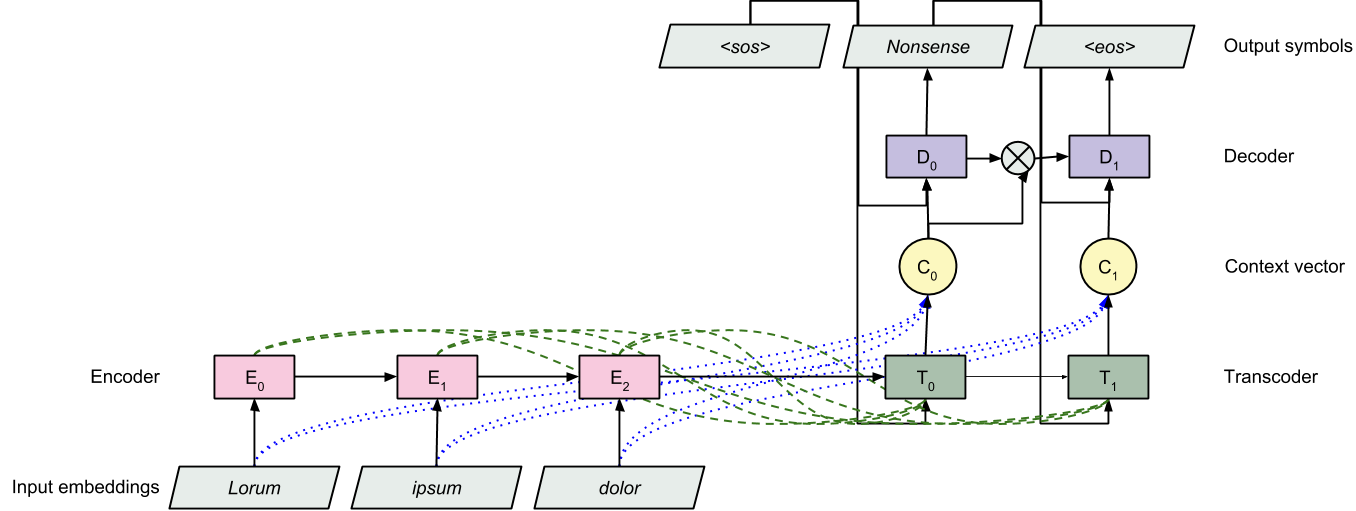
\includegraphics[width=0.9\linewidth]{model}
\caption{Schematic overview of the seq2attn architecture.}
\end{figure}
In summary, the proposed seq2attn model could be explained as a combination of four adaptations of the standard seq2seq architecture with attention. 

\begin{enumerate}
\item The decoder receives information of the encoder solely through context vectors produced by a specialized attention module called the transcoder. This is to stimulate a focused processing of input tokens.
\item The context vectors produced by the decoder are weighted sums over the encoder's \emph{embeddings} instead of its hidden states.
\item The weights with which the embeddings are combined into a context vector are the result not of a Softmax function, but of a Gumbel-Softmax function with the Straight-Through (ST) Estimator  to enforce the use of a single embedding per decoder step.
\item The hidden states of the decoder are element-wise multiplied with the context vectors produced by the transcoder to further enforce the use of the attention module.
\end{enumerate}

\end{block}

%----------------------------------------------------------------------------------------
%	RESULTS
%----------------------------------------------------------------------------------------

\begin{block}{Results: Accuracies}
	
	\begin{table}
		\centering
		\begin{center}
			\begin{tabular}{l|lll}
				& \multicolumn{1}{c}{\begin{tabular}[c]{@{}c@{}}held-out\\ inputs\end{tabular}}
				& \multicolumn{1}{c}{\begin{tabular}[c]{@{}c@{}}held-out\\ compositions\end{tabular}} 
				& \multicolumn{1}{c}{\begin{tabular}[c]{@{}c@{}}held-out\\ tables\end{tabular}} \\ \hline
				Baseline & 38.25 $\pm$ 0.04 & 43.28 $\pm$ 0.09 & 7.86 $\pm$ 0.02 \\
				Seq2attn & \textbf{100 $\pm$ 0.00} & \textbf{100 $\pm$ 0.00} & \textbf{100 $\pm$ 0.00}
			\end{tabular}%
		\end{center}
		\caption{Average sequence accuracies and standard deviations of the baseline seq2seq and seq2attn models on all lookup tables test sets.}
		\label{tab:lookup-accuracies}
	\end{table}
	
	\begin{figure}
		\begin{tikzpicture}
\begin{axis}[
    ybar,
    axis x line*=bottom,
    axis y line*=left,
    symbolic x coords={1,2,4,8,16,32,64,128,256,512,1024},
    anchor=above north,
    ymax=100,
    tickwidth=6pt,
    bar width=12pt,
    enlarge x limits = 0.06,
    xtick=data,
    xticklabel style={align=center, font=\small},
    ylabel=sequence accuracy,
    xlabel=Number of training examples containing \texttt{look around right},
    % legend pos=north east,
    %legend columns=2,
    %legend style={at={(0.85,1.27)}},
    height=0.4\linewidth,
    width=0.6\linewidth
    ]
        \addplot [style={fill=green_mtplotlib},error bars/.cd, y dir=both,y explicit]  
        table [x=test set, y=mean,y error=conf, col sep=comma,] {./Data/scan_exp3_seq2attn.csv};	

        \addplot [pattern=north east lines, pattern color=red,error bars/.cd, y dir=both,y explicit]  
        table [x=test set, y=mean,y error=conf, col sep=comma,] {./Data/scan_exp3_baseline.csv};
        
        %\legend{seq2attn,baseline}	
\end{axis}
\end{tikzpicture}

		\caption{Mean sequence accuracies on experiment 3 of the SCAN task while testing on sequences containing \texttt{jump around right}.}
	\end{figure}
	
\end{block}

%----------------------------------------------------------------------------------------

\end{column} % End of the first column

\begin{column}{.03\textwidth}\end{column} % Empty spacer column
 
\begin{column}{.465\textwidth} % The second column

%------------------------------------------------

\begin{block}{Results: Attention patterns}

\begin{figure}
    \centering
	\begin{subfigure}{.33\linewidth}
		\centering
		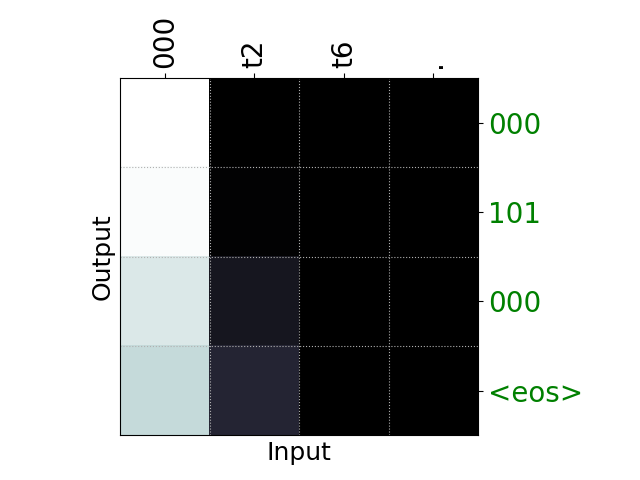
\includegraphics[width=0.80\linewidth,trim={2cm 0cm 1cm 0cm},clip]{Figures/attn_baseline_lookup_distributed}
		\caption{seq2seq}
		\label{fig:attn_baseline_lookup_heldout_input1}
	\end{subfigure}%
	\begin{subfigure}{.33\linewidth}
		\centering
		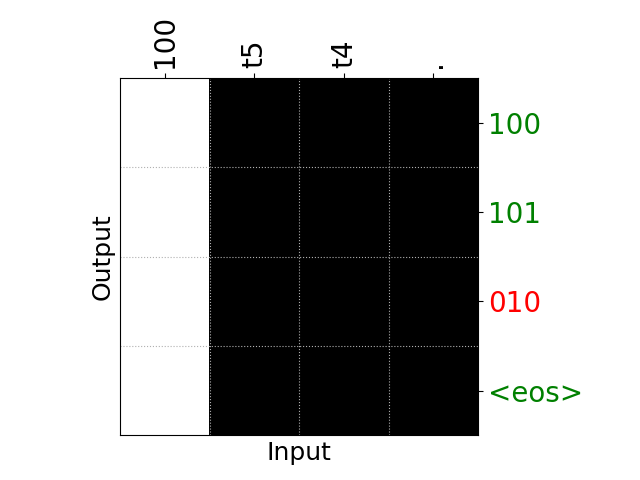
\includegraphics[width=0.80\linewidth,trim={2cm 0cm 1cm 0cm},clip]{Figures/attn_baseline_lookup_sparse}
		\caption{seq2seq}
		\label{fig:attn_baseline_lookup_heldout_input2}
	\end{subfigure}%
	\begin{subfigure}{.33\linewidth}
		\centering
		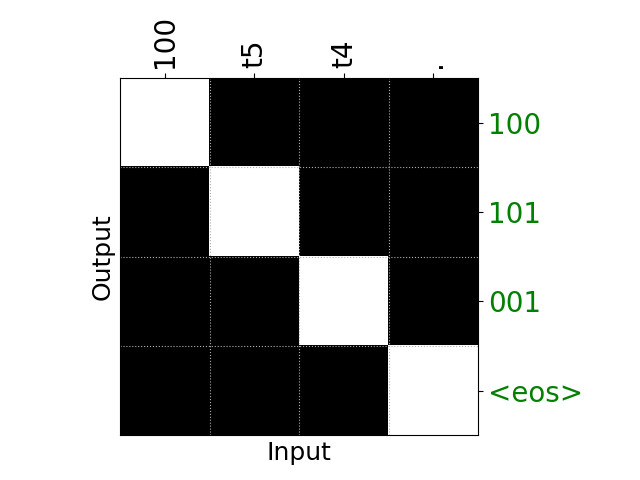
\includegraphics[width=0.80\linewidth,trim={2cm 0cm 1cm 0cm},clip]{Figures/attn_seq2attn_lookup}
		\caption{seq2attn}
		\label{fig:attn_seq2attn_lookup_heldout_input}
	\end{subfigure}
	\caption{Examples of modeled attention patterns on held-out input examples of the lookup tables domain.}
	\label{fig:attn_lookup}
\end{figure}

\begin{figure}
	\centering
	\begin{subfigure}{.33\linewidth}
		\centering
		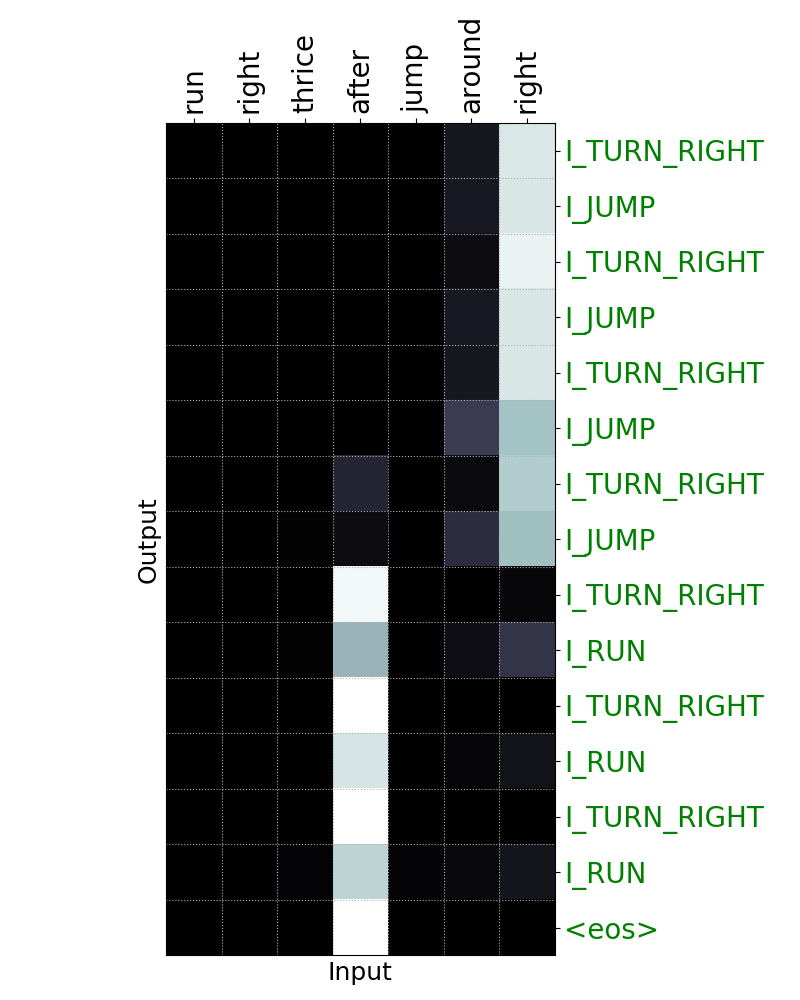
\includegraphics[width=0.77\linewidth,trim={3cm 0cm 0.9cm 0cm},clip]{Figures/attn_baseline_scan_1}
		\caption{seq2seq}
		\label{fig:scan_attn_baseline}
	\end{subfigure}%
	\begin{subfigure}{.33\linewidth}
		\centering
		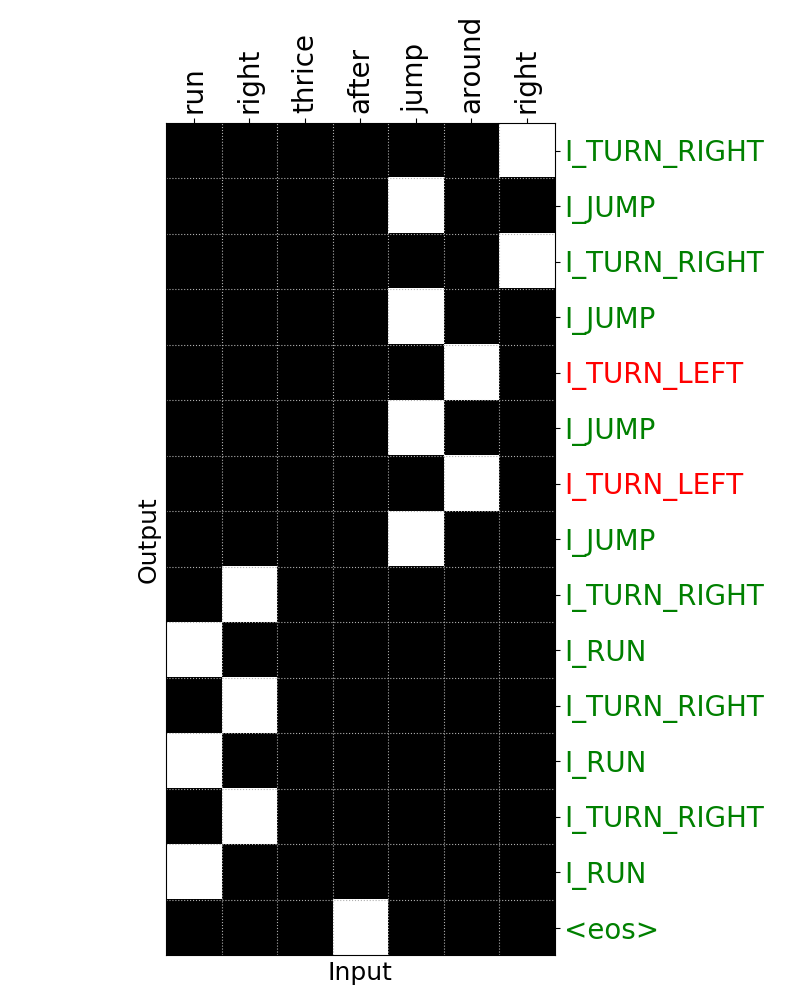
\includegraphics[width=0.77\linewidth,trim={3cm 0cm 0.9cm 0cm},clip]{Figures/attn_seq2attn_scan_incorrect}
		\caption{seq2attn}
		\label{fig:scan_attn_seq2attn_incorrect}
	\end{subfigure}%
	\begin{subfigure}{.33\linewidth}
		\centering
		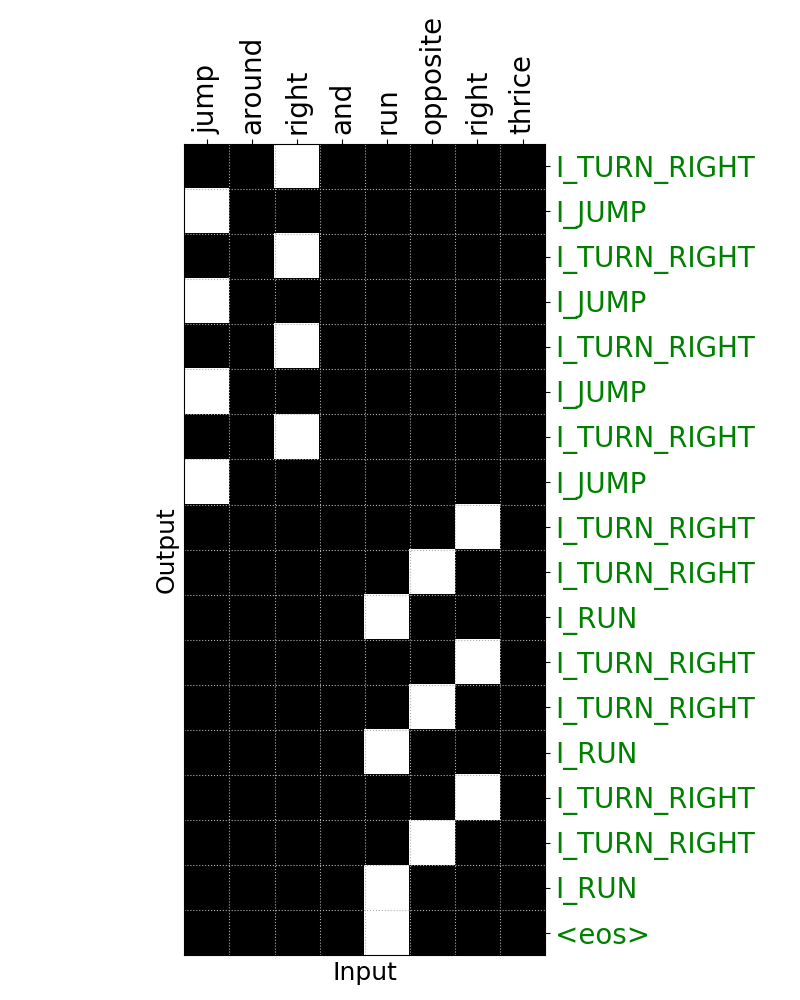
\includegraphics[width=0.77\linewidth,trim={3cm 0cm 0.9cm 0cm},clip]{Figures/attn_seq2attn_scan_correct}
		\caption{seq2attn}
		\label{fig:scan_attn_seq2attn_correct}
	\end{subfigure}
	\caption{Examples of attention patterns in the SCAN domain. Note how seq2attn models the output incorrectly when the attention patterns are incorrect.}
	\label{fig:scan_attn}
\end{figure}

\end{block}


%----------------------------------------------------------------------------------------
%	OERGENERALIZATION
%----------------------------------------------------------------------------------------

\begin{block}{Results: Overgeneralization}
	
We suspect that compositional generalization leads to more  \emph{overgeneralization}. This is a phenomenon where a learner generalizes rules even to exceptions where these rules do not apply. For the lookup tables task, we test this by making the output of \texttt{\textit{x} t1 t2} random for 3 of the 8 bit-strings.
\begin{figure}
	\centering
	\begin{subfigure}{0.5\linewidth}
	\documentclass{standalone}
\usepackage{graphicx}
\usepackage[mode=buildnew]{standalone}
\usepackage{tikz}
\usepackage{nicefrac}
\usepackage{pgfplots}
\pgfplotsset{
    discard if not/.style 2 args={
        x filter/.code={
            \edef\tempa{\thisrow{#1}}
            \edef\tempb{#2}
            \ifx\tempa\tempb
            \else
            \def\pgfmathresult{inf}
            \fi
        }
    },ymin=0,ymax=1,
    compat=newest
}
\usepgfplotslibrary{fillbetween}
\usepackage{pgfplotstable}
\pgfplotsset{compat=1.13}
\usepgfplotslibrary{colormaps} % LATEX and plain TEX
\definecolor{awesome}{rgb}{1.0, 0.13, 0.32}
\definecolor{magenta_mtplotlib}{rgb}{1.0, 0.0, 1.0}
\definecolor{green_mtplotlib}{rgb}{0.0, 0.5019607843137255, 0.0}
\definecolor{blue_mtplotlib}{rgb}{0.0, 0.0, 1.0}

\begin{document}

\begin{tikzpicture}
\begin{axis}[
    smooth,
    anchor=above north,
    width=0.8\linewidth,height=0.6\linewidth,
    ymax=1,
    xmax=30,
    xmin=0,
    xtick={0, 5, 10, 15, 20, 25, 30, 35, 40, 45, 50},
    tickwidth=2pt,
    ylabel=sequence accuracy,
    xlabel=epochs,
    ytick={0,0.125,0.25,0.375,0.5,0.6250,0.75,0.8750,1.0},
    yticklabels={${\nicefrac{0}{8}}$,$\nicefrac{1}{8}$,$\nicefrac{2}{8}$,$\nicefrac{3}{8}$,$\nicefrac{4}{8}$,$\nicefrac{5}{8}$,$\nicefrac{6}{8}$,$\nicefrac{7}{8}$,$\nicefrac{8}{8}$ },
    axis on top,
    ticklabel style = {font=\small}
    ]

        \addplot [name path=upper,draw=none] table[x=epochs, y expr=\thisrow{average}+\thisrow{confidence}] {Data/corruption-lookup-baseline.csv};
        \addplot [name path=lower,draw=none] table[x=epochs, y expr=\thisrow{average}-\thisrow{confidence}] {Data/corruption-lookup-baseline.csv};
        \addplot [fill=green_mtplotlib!10] fill between[of=upper and lower];
        \addplot [mark=none, color=green_mtplotlib, line width=1pt] table [x=epochs,y=average] {Data/corruption-lookup-baseline.csv};
        \node at (axis cs:14.5,0.75) [anchor=north east, font=\small] {overgen.};
        \addplot [color=red!80, line width=1pt, style=dashed] coordinates{(0,0.625) (30,0.625)};
\end{axis}
\end{tikzpicture}
\end{document}

	\caption{seq2seq}
\end{subfigure}%
\begin{subfigure}{0.5\linewidth}
	\documentclass{standalone}
\begin{document}

\begin{tikzpicture}
\begin{axis}[
    smooth,
    width=0.8\linewidth,height=0.6\linewidth,
    anchor=above north,
    ymax=1,
    xmax=30,
    xmin=0,
    xtick={0, 5, 10, 15, 20, 25, 30, 35, 40, 45, 50},
    tickwidth=2pt,
    xlabel=epochs,
    ylabel={{sequence accuracy}},
    ytick={0,0.125,0.25,0.375,0.5,0.6250,0.75,0.8750,1.0},
    yticklabels={$\textcolor{black}{\nicefrac{0}{8}}$,$\textcolor{black}{\nicefrac{1}{8}}$,$\textcolor{black}{\nicefrac{2}{8}}$,$\textcolor{black}{\nicefrac{3}{8}}$,$\textcolor{black}{\nicefrac{4}{8}}$,$\textcolor{black}{\nicefrac{5}{8}}$,$\textcolor{black}{\nicefrac{6}{8}}$,$\textcolor{black}{\nicefrac{7}{8}}$,$\textcolor{black}{\nicefrac{8}{8}}$ },
    axis on top,
    ticklabel style = {font=\small}
    ]

        \addplot [name path=upper,draw=none] table[x=epochs, y expr=\thisrow{average}+\thisrow{confidence}] {Data/corruption-lookup-seq2attn.csv};
        \addplot [name path=lower,draw=none] table[x=epochs, y expr=\thisrow{average}-\thisrow{confidence}] {Data/corruption-lookup-seq2attn.csv};
        \addplot [fill=green_mtplotlib!10] fill between[of=upper and lower];
        \addplot [mark=none, color=green_mtplotlib, line width=1pt] table [x=epochs,y=average] {Data/corruption-lookup-seq2attn.csv};
        \node at (axis cs:29.5,0.75) [anchor=north east, font=\small] {overgen.};
        \addplot [color=red!80, line width=1pt, style=dashed] coordinates{(0,0.625) (30,0.625)};
\end{axis}
\end{tikzpicture}
\end{document}

	\caption{seq2attn}
\end{subfigure}
\caption{Average accuracies on the \emph{original targets} for the eight inputs in composition \texttt{\textit{x} t1 t2}. As three of these compositions are exceptions, we refer to accuracy higher than $\nicefrac{5}{8}$ as overgeneralization.}
\label{fig:corruption-lookup}
\end{figure}
	
\end{block}

%----------------------------------------------------------------------------------------
%	TASKS
%----------------------------------------------------------------------------------------

\begin{block}{Tasks}
	
	\begin{itemize}
		\item Lookup Tables
		\begin{itemize}
			\item The input sequences consist in a three-bit string followed by a series of function identifiers for lookup tables. The objective is to apply these bijective functions over the (intermediate) outputs successively
			\item Example: \texttt{001} \texttt{t1} \texttt{t2} $\rightarrow$ \texttt{001} \texttt{010} \texttt{111}
		\end{itemize}
		
		\item SCAN
		\begin{itemize}
			\item The input consists in one or two sub-sequences which can be joined by the conjunctives \texttt{and} or \texttt{after}. Each sub-sequence contains a primitive command and possibly modifiers that act on this command. The learner must interpret the commands and mentally apply them in a 2D game grid.
			\item Example: \texttt{jump after walk left twice} $\rightarrow$ \texttt{I\_TURN\_LEFT I\_WALK I\_TURN\_LEFT I\_WALK I\_JUMP}
		\end{itemize}
		
	\end{itemize}
	
\end{block}


%----------------------------------------------------------------------------------------
%	CONCLUSION
%----------------------------------------------------------------------------------------

\begin{block}{Conclusion}

\begin{itemize}
	\item increased general performance on specialized tasks indicate improved compositional generalization by seq2attn.
	\item The general ideas implemented could be extended to several variants of encoder-decoder architectures.
	\item Sparser attentional patterns improve interpretability of the found solutions,
	\item Preliminary results show neither increased or decreased performance on NMT (without the Sraight-Through estimator of Gumbel-Softmax)
	\item Strictly sparse attention vectors might limit the expressiveness of the model. Possible improvements may be made by research on alternatives methods.
\end{itemize}

\end{block}

\end{column} % End of the second column

\begin{column}{.015\textwidth}\end{column} % Empty spacer column

\end{columns} % End of all the columns in the poster

\end{frame} % End of the enclosing frame

\end{document}